\chapter{Implementation of Direct GPU-FPGA Communication}
\label{section:implementation}

\section{Environment}

As simulation environment I am using V-REP 3.4.0\cite{Rohmer2013}

SNN controllers are implemented using NEST simulator 2.14.0\cite{Peyser2017}

The simulation and the python controller communicate over ROS kinetic\cite{}



\begin{lstlisting}[label=listing:example_code, caption=example]
code = example
\end{lstlisting}

\section{Setup}

\begin{figure}
	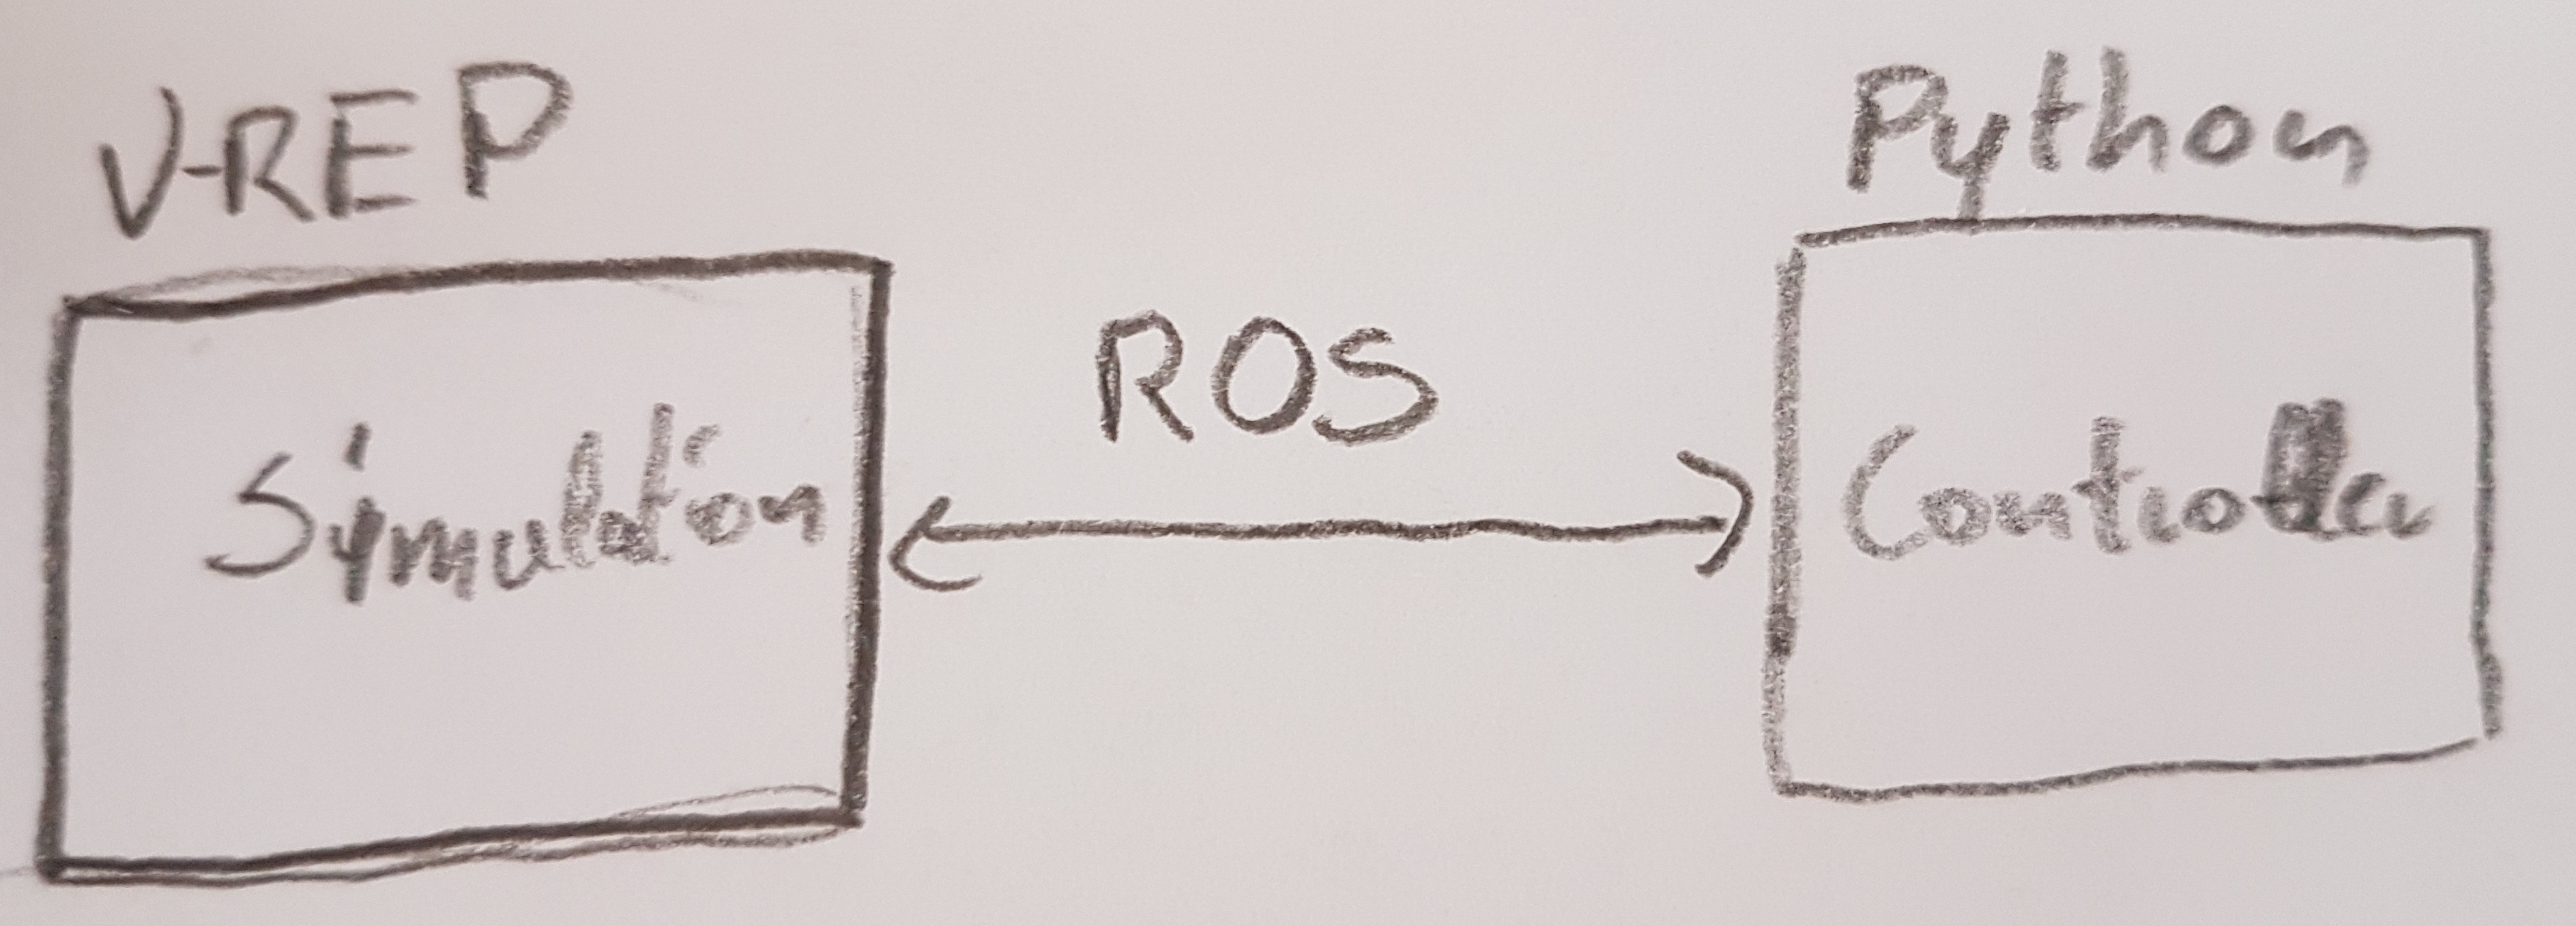
\includegraphics[width=\linewidth]{images/setup.jpg}
	\caption{The two main components and the communication channel}
	\label{fig:setup}
\end{figure}


This section gives a high overview of the experiment. In figure \ref{fig:setup} you can see that there are two main components. First we have the simulation made with V-Rep witch contains the snake like robot and the environment. The environment is made out of a target ball the snake will learn to follow and obstacles in the form of walls. The snake moves according to the movement model from section \ref{section:model}. The second important component is the python controller that will learn to manoeuvre the snake through the environment successfully. The structure of the controller is described in detail in the following section. It contains SNN that will solve a target following and an obstacle avoidance task. The SNN are implemented using the NEST simulator. Both components communicate with each other using ROS. They are both ROS nodes and can exchange messages over the ROS Topic messaging protocol.


\section{Controller}

\begin{figure}
	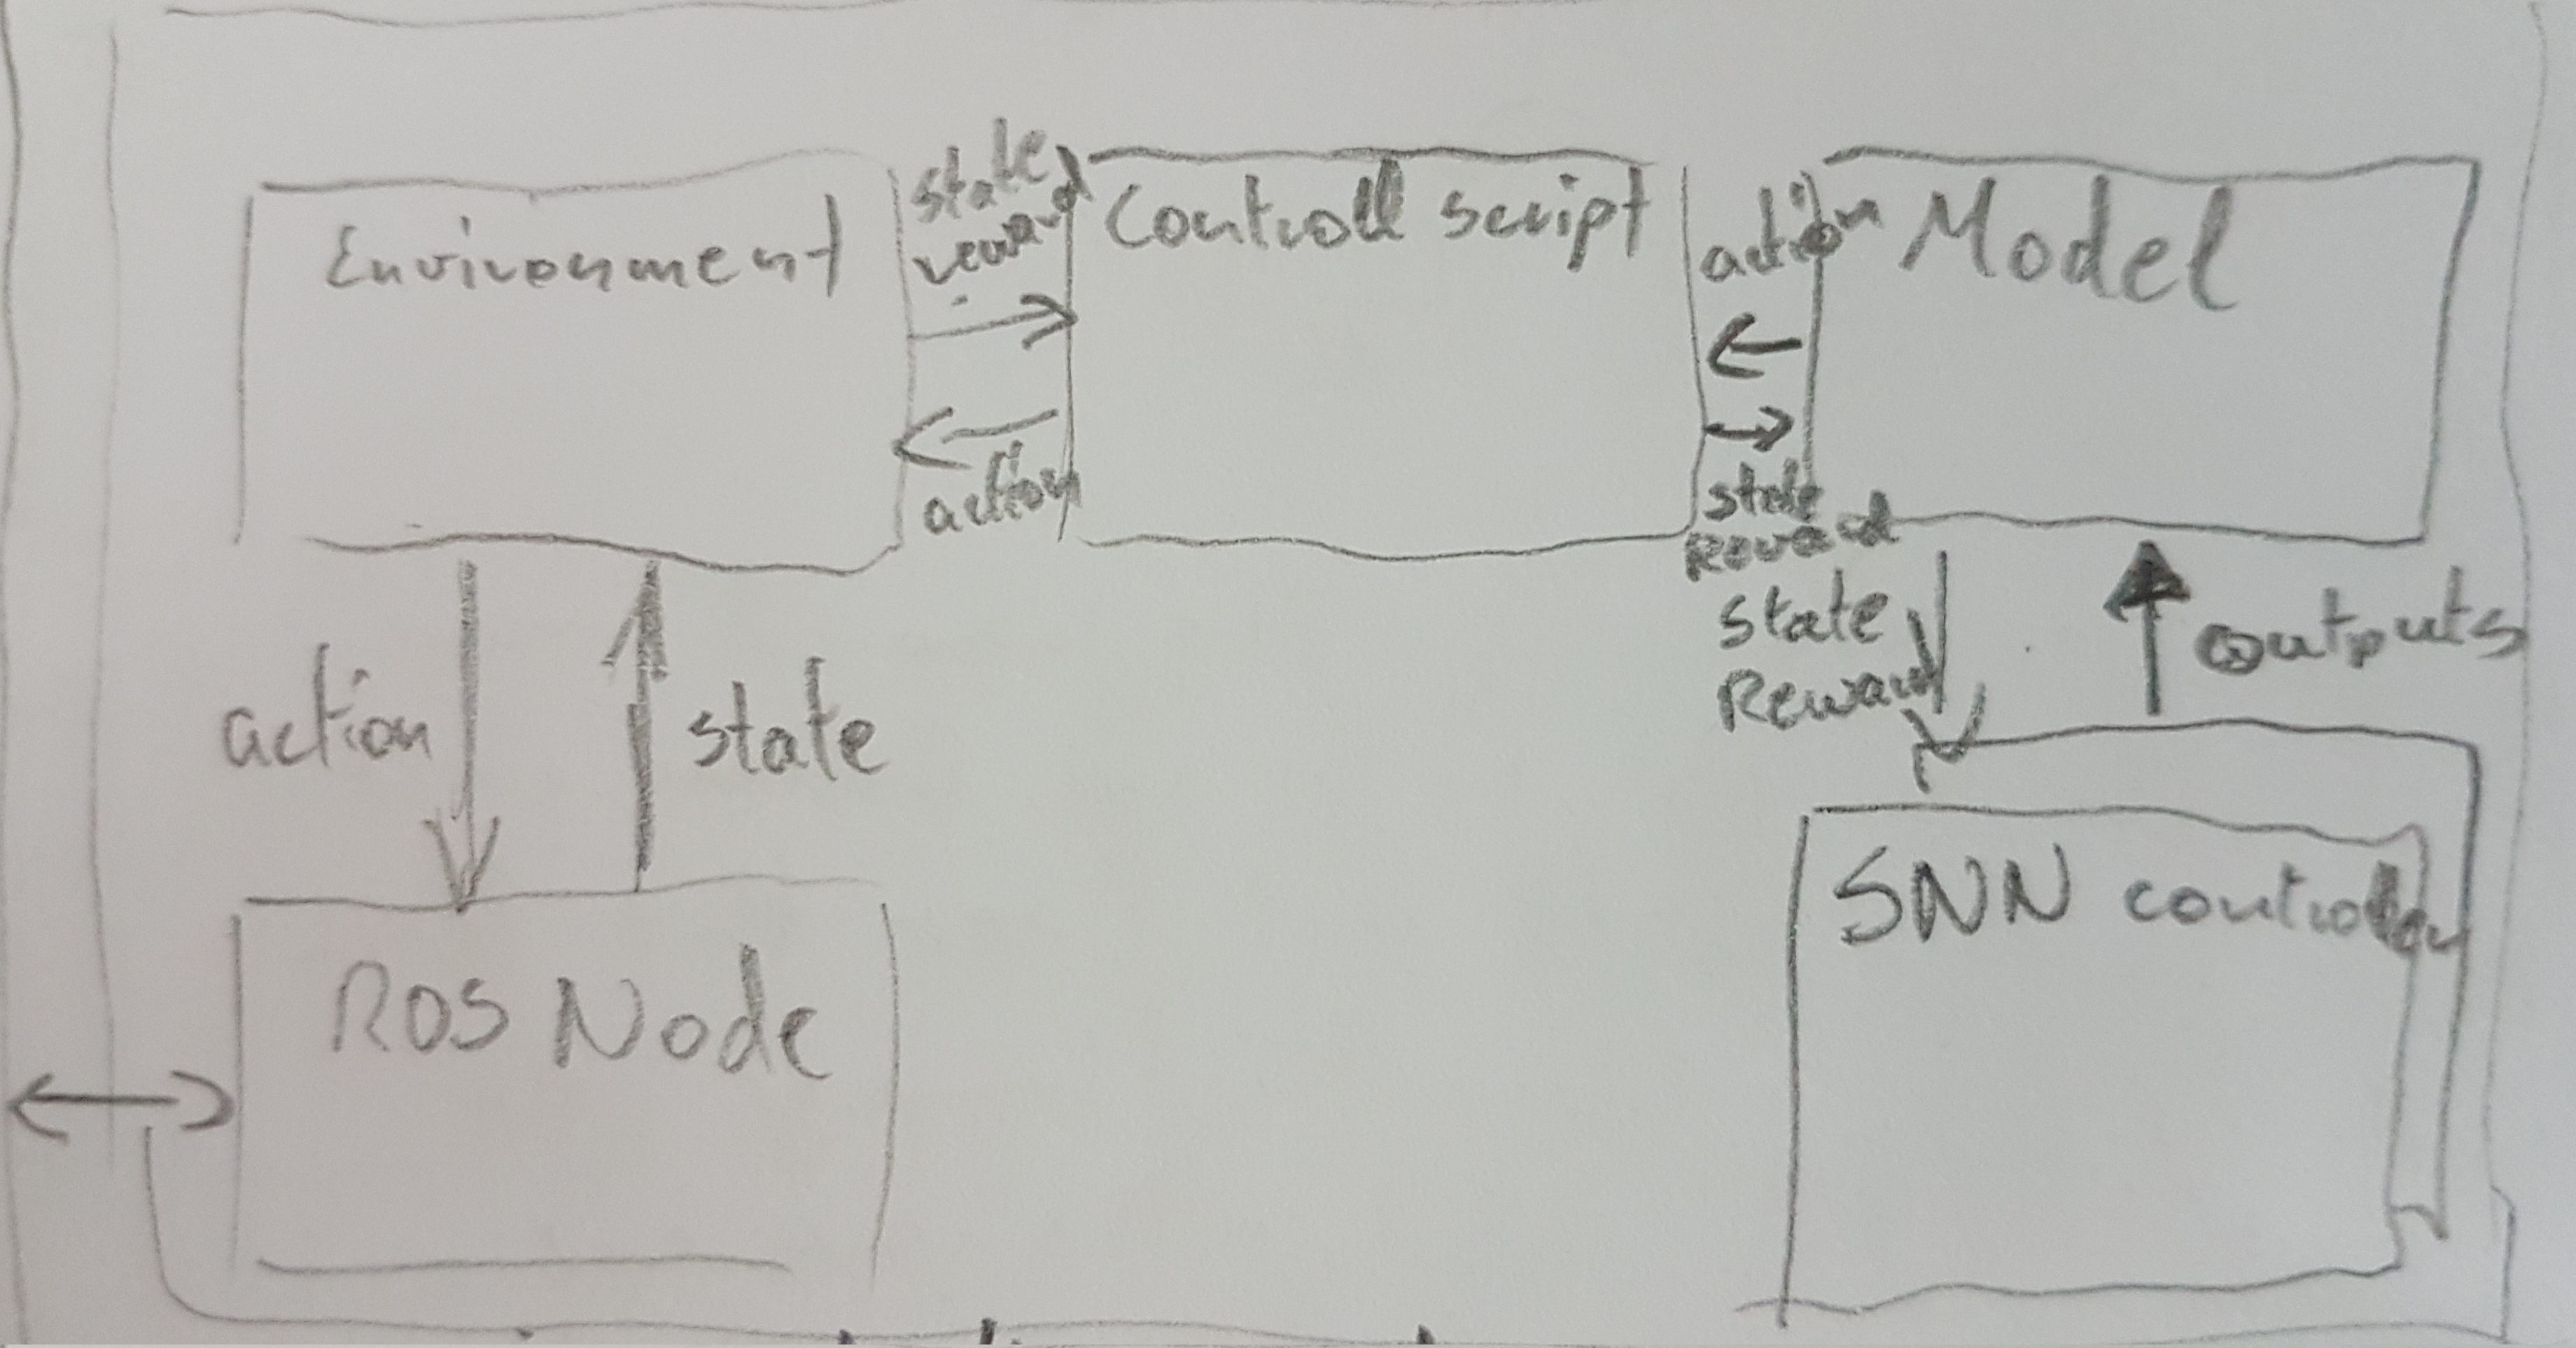
\includegraphics[width=\linewidth]{images/controller.jpg}
	\caption{Architecture of the python controller}
	\label{fig:controller}
\end{figure}

The controller is written in python and distributed over 5 components as can be seen in figure \ref{fig:controller}. Each is implemented in one file. The responsibilities are distributed as follows:

\begin{itemize}
	\item \textbf{Simulation}: The simulation class implements a ROS node and represents the simulation for the controller. All communication with V-Rep goes through this class. Messages are processed and then send to the simulation. Received information gets preprocessed before they are used. It contains the state of the environment as the robot is able to perceive it at a certain moment.
	\item \textbf{Environment}: This class uses the information form the simulation to create a state object. The reward for each output neuron in the SNN's are also calculated here. This class manages changes in the environment like resets.
	\item \textbf{Controll scripts}: They are controlling the experiment flow like if and witch network gets trained. It will also collect data from the environment and the model and save it for later analysis. Examples for these scripts are the training script that will train one model or the controll script that will execute one model for evaluation.
	\item \textbf{Model}: Here the state is feed to the SNN to recive outputs witch then will be interpreted to cosntruct an action that the snake in the simulation will perform.
	\item \textbf{SNN}: The implementation of the SNN network using Nest.
\end{itemize}

\section{Sensors}

\begin{figure}
	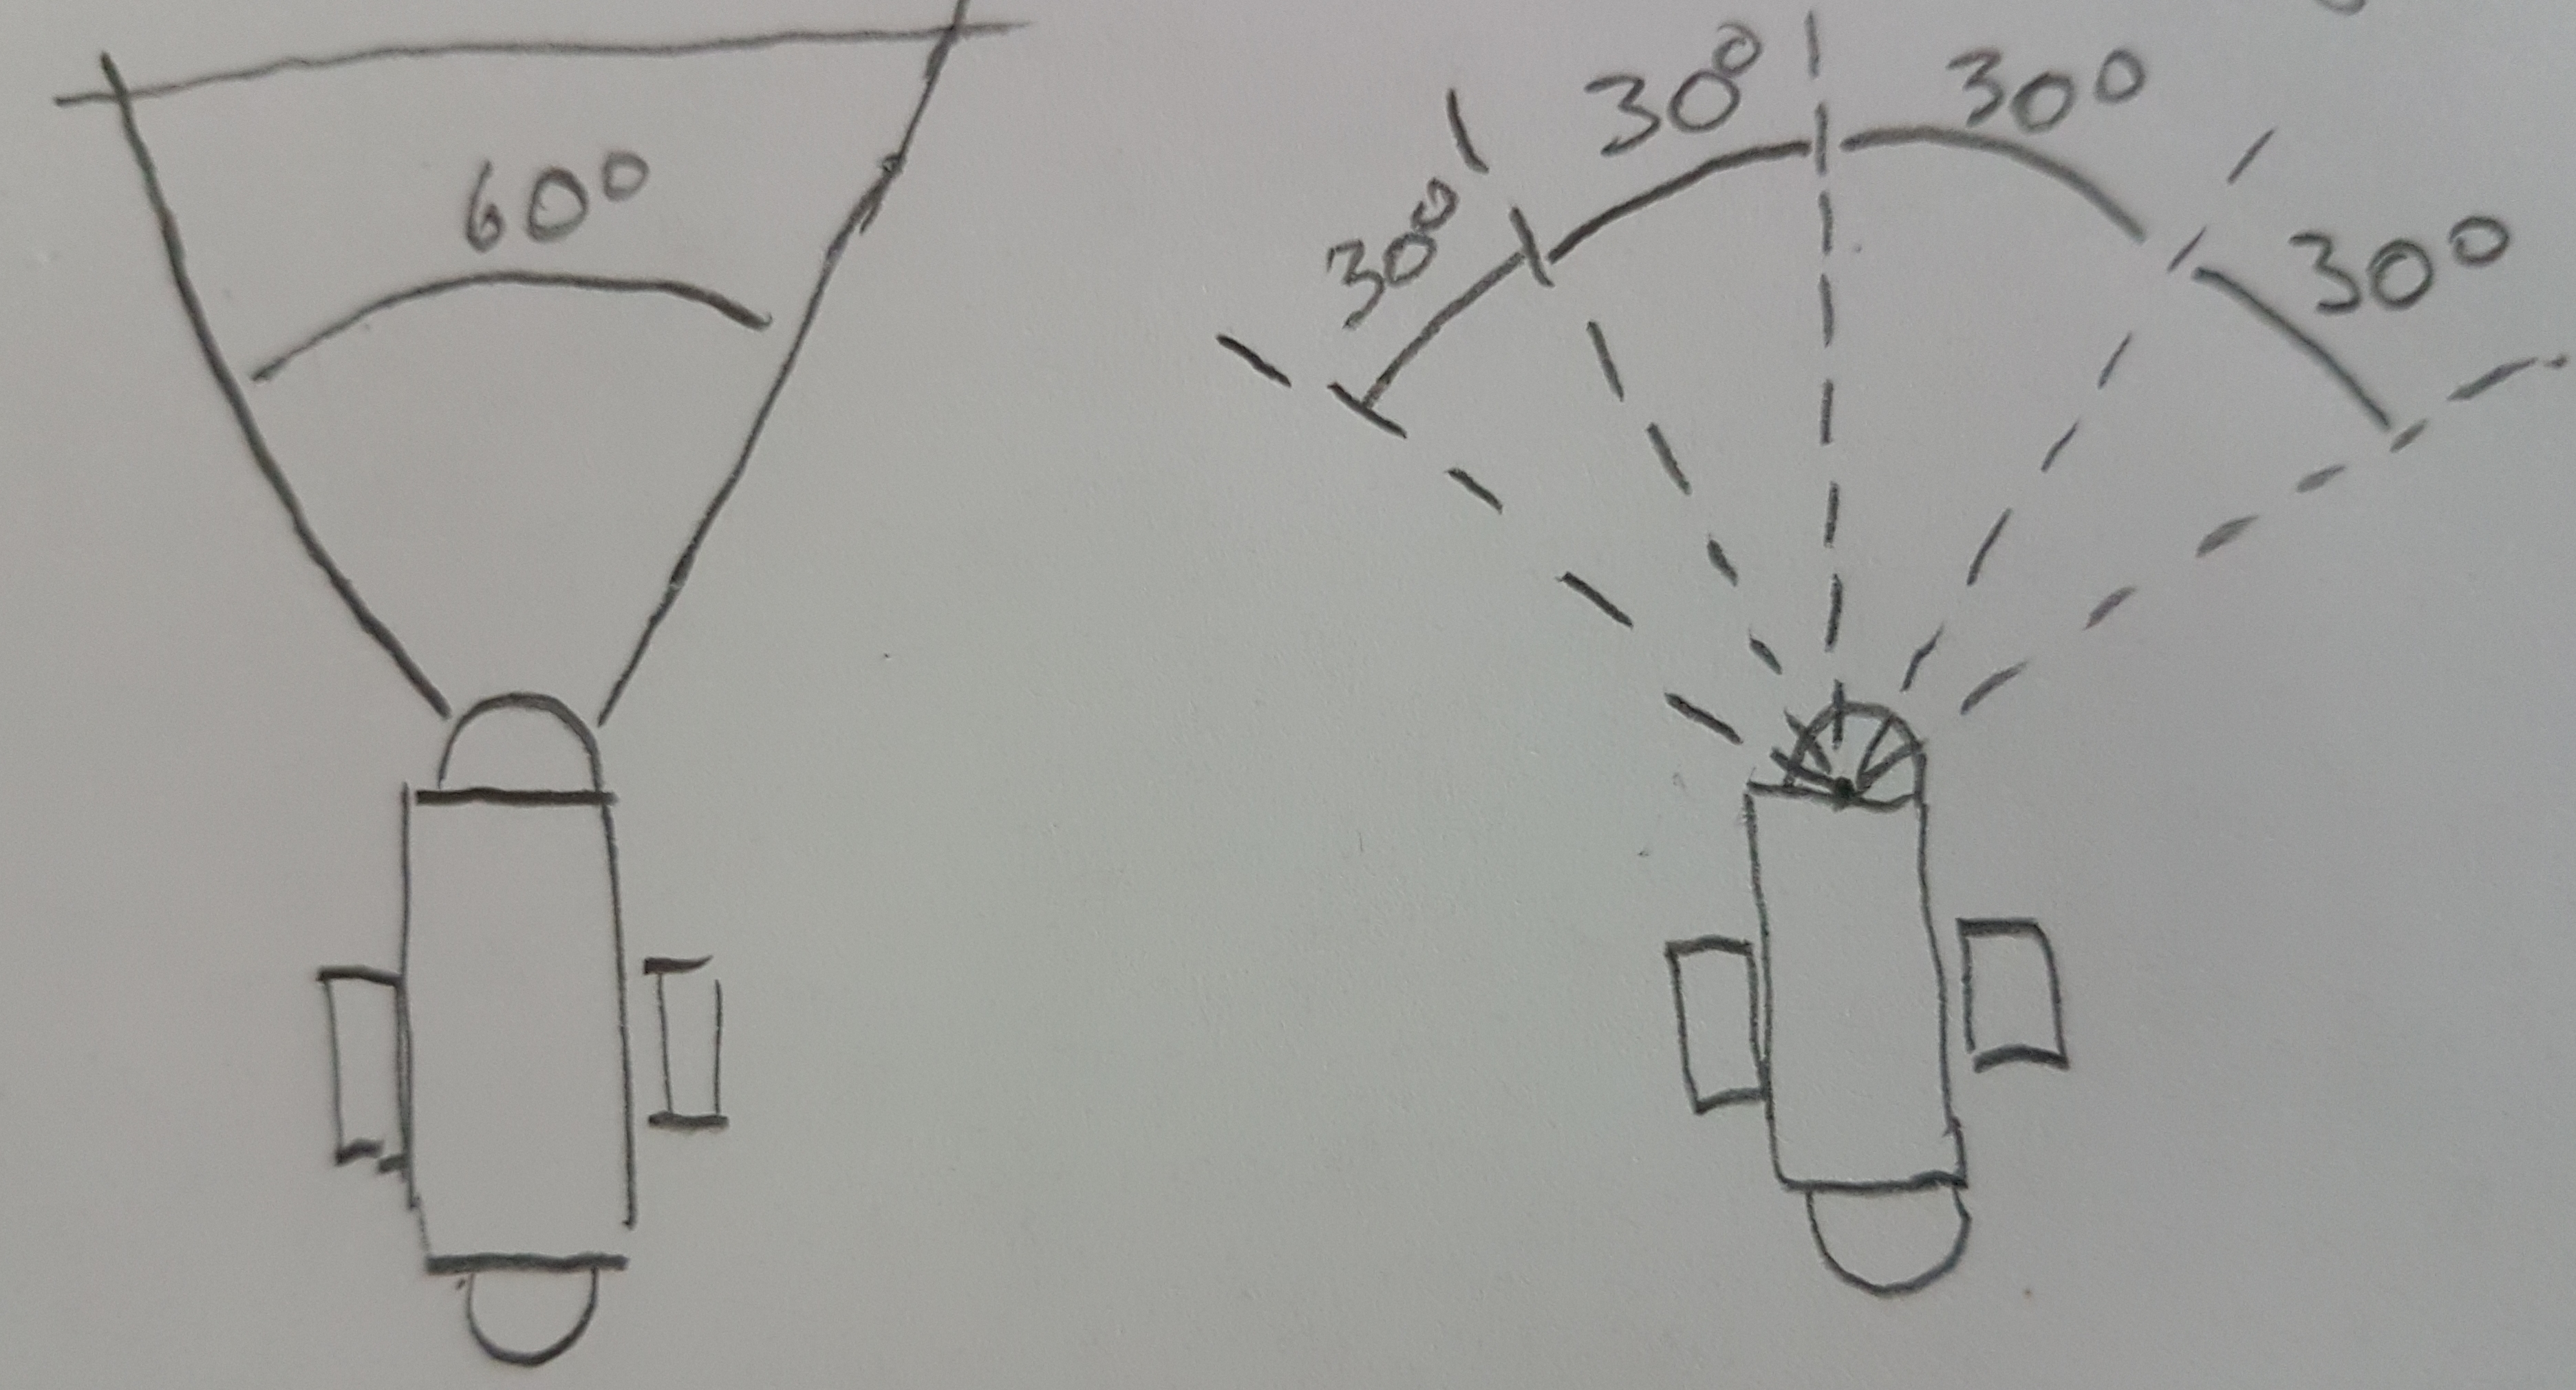
\includegraphics[width=\linewidth]{images/sensors.jpg}
	\caption{a. Shows the vision sensor of the snake that is fixed on the snake head. b. Shows the five proximity sensors on the snake. The one in the middle senses the target while the other four sense obstacles.}
	\label{fig:sensors}
\end{figure}

The sensors are all mounted on the head of the snake as shown in figure \ref{fig:sensors}. The first sensor is the vision sensor used for target following. It is a infra-red vision sensor with a field of view of 60°. It returns a 32x32 Pixel image of the environment. The only thing the camera can distinguish is the warm target since everything else has the same temperature. Then there are 5 proximity sensors on the snake head. The first one looks straight ahead and measures the distance to the target in a wide ark and is used to determine the speed of the snake. The other four have offsets of $\pm30°$ and $\pm60°$ respectively. They can sense obstacles in a straight line.

\section{Target Following Controller}

\begin{figure}
	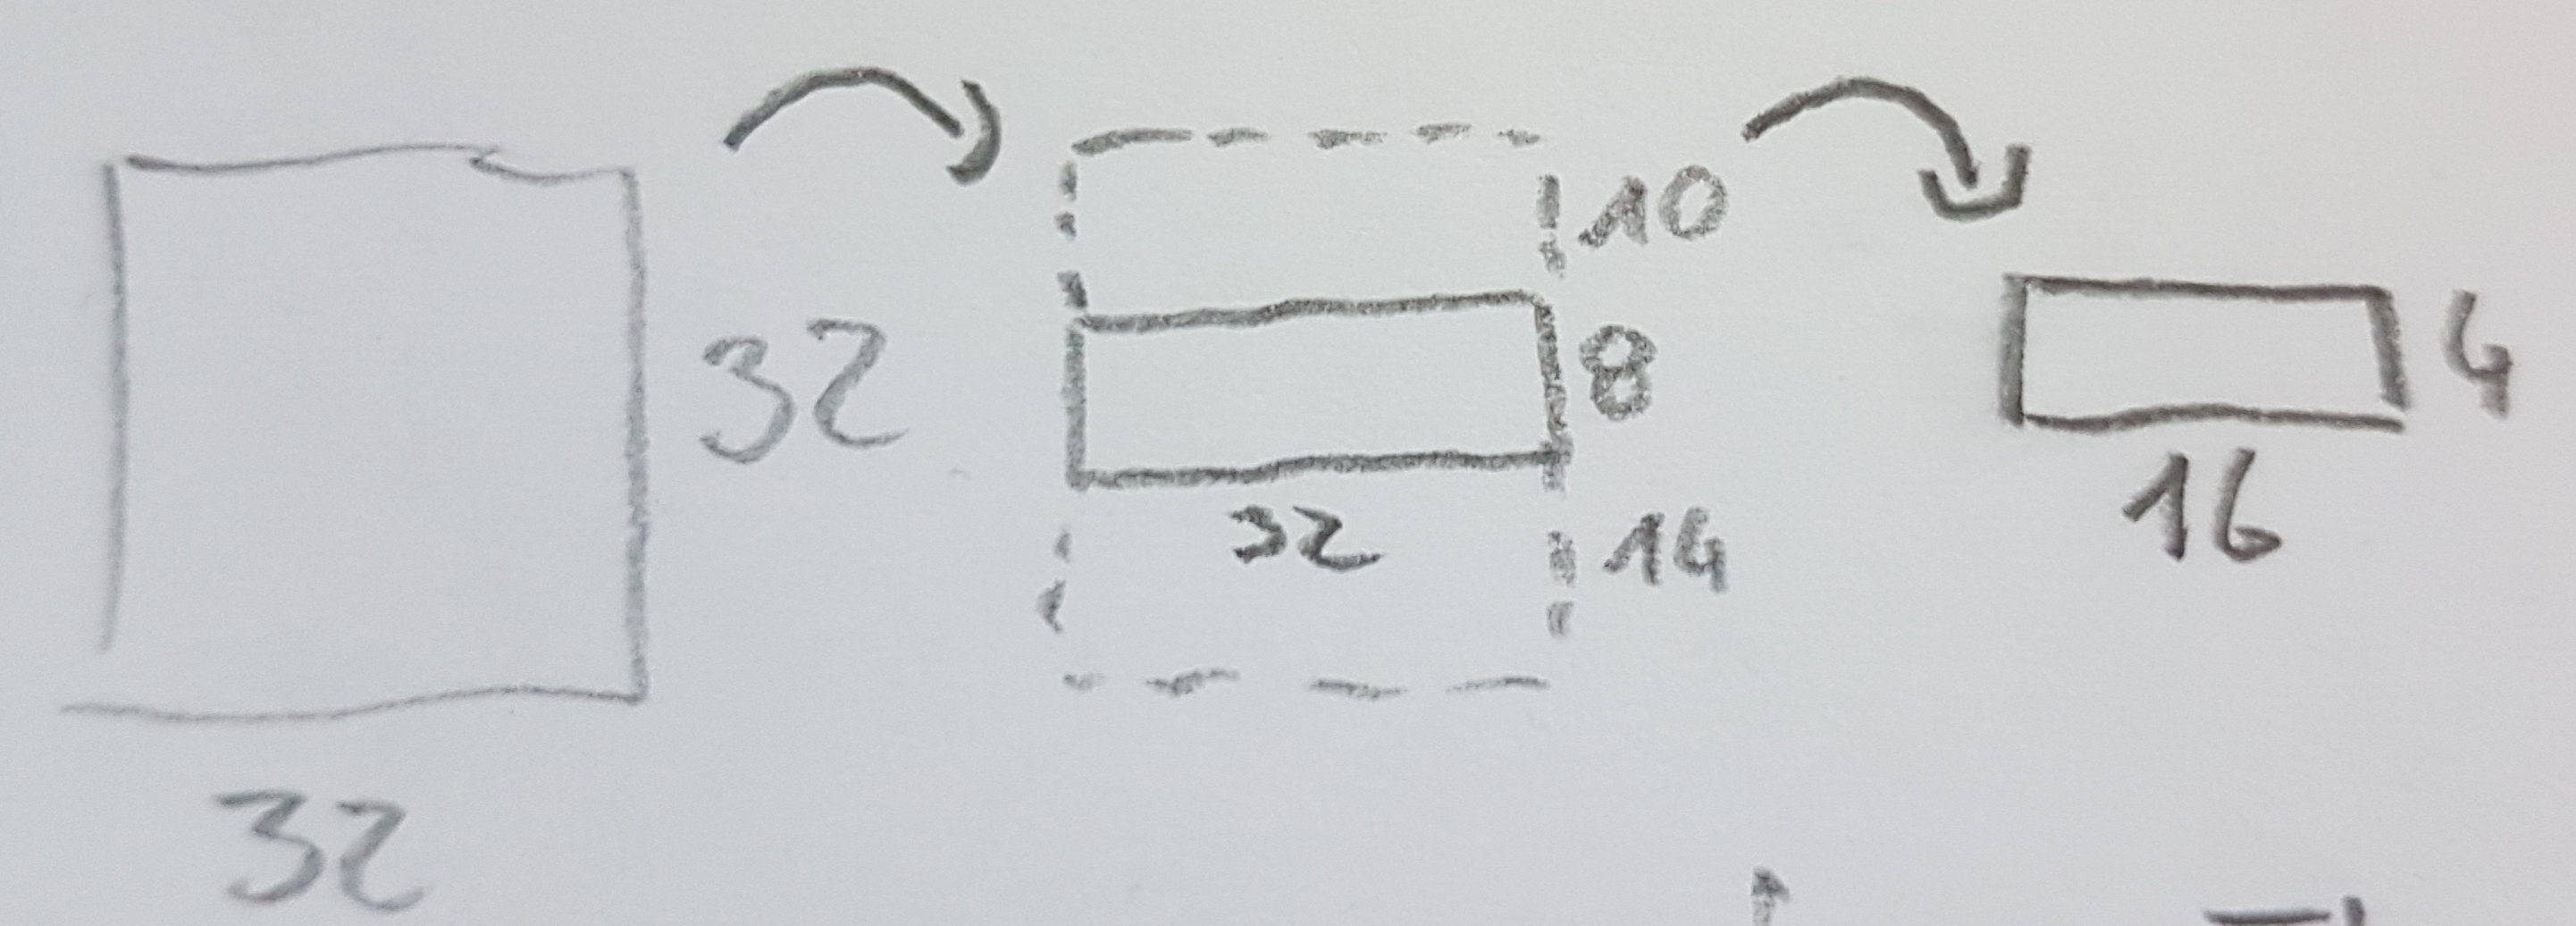
\includegraphics[width=\linewidth]{images/img_pre.jpg}
	\caption{a. 32x32 Infra red image b. cut out 32x8 pixel part c. 16x4 pixel image by averaged over 2x2 pixel patches}
	\label{fig:img_pre}
\end{figure}

The goal of the target following controller is it to successfully follow a target trough the environment. In our simulation the target is represented by a warm ball that can be seen by the infra red camera on the head of the snake. The input for the controller is a infra red image with size 32x32 pixel. The preprocesing of the image has 2 steps as shown in figure \ref{fig:img_pre} before it gets feed to the network. First the top and bottom part gets removed, since these will only see the floor and ceiling. Then the image gets down sampled by taking the average over 2x2 pixels. The resulting image is now 16x4 and gets scaled and mapped to poison firing rates witch are the input for the 64 input neurons for the network. The network has a  simple feed forward architecture shown in figure \ref{fig:follw_arch} with 64 input neurons and 2 output neurons. The input gets transformed to spike trains by poison distributed spike generators. The output of the Network is the ammount of spikes the left and right neuron produce. The right neuron gets assigned reward proportional to the angle between the direction the snake looks and the target. THe left neuron gets assigned the negative of the reward for the right neuron.

\begin{figure}
	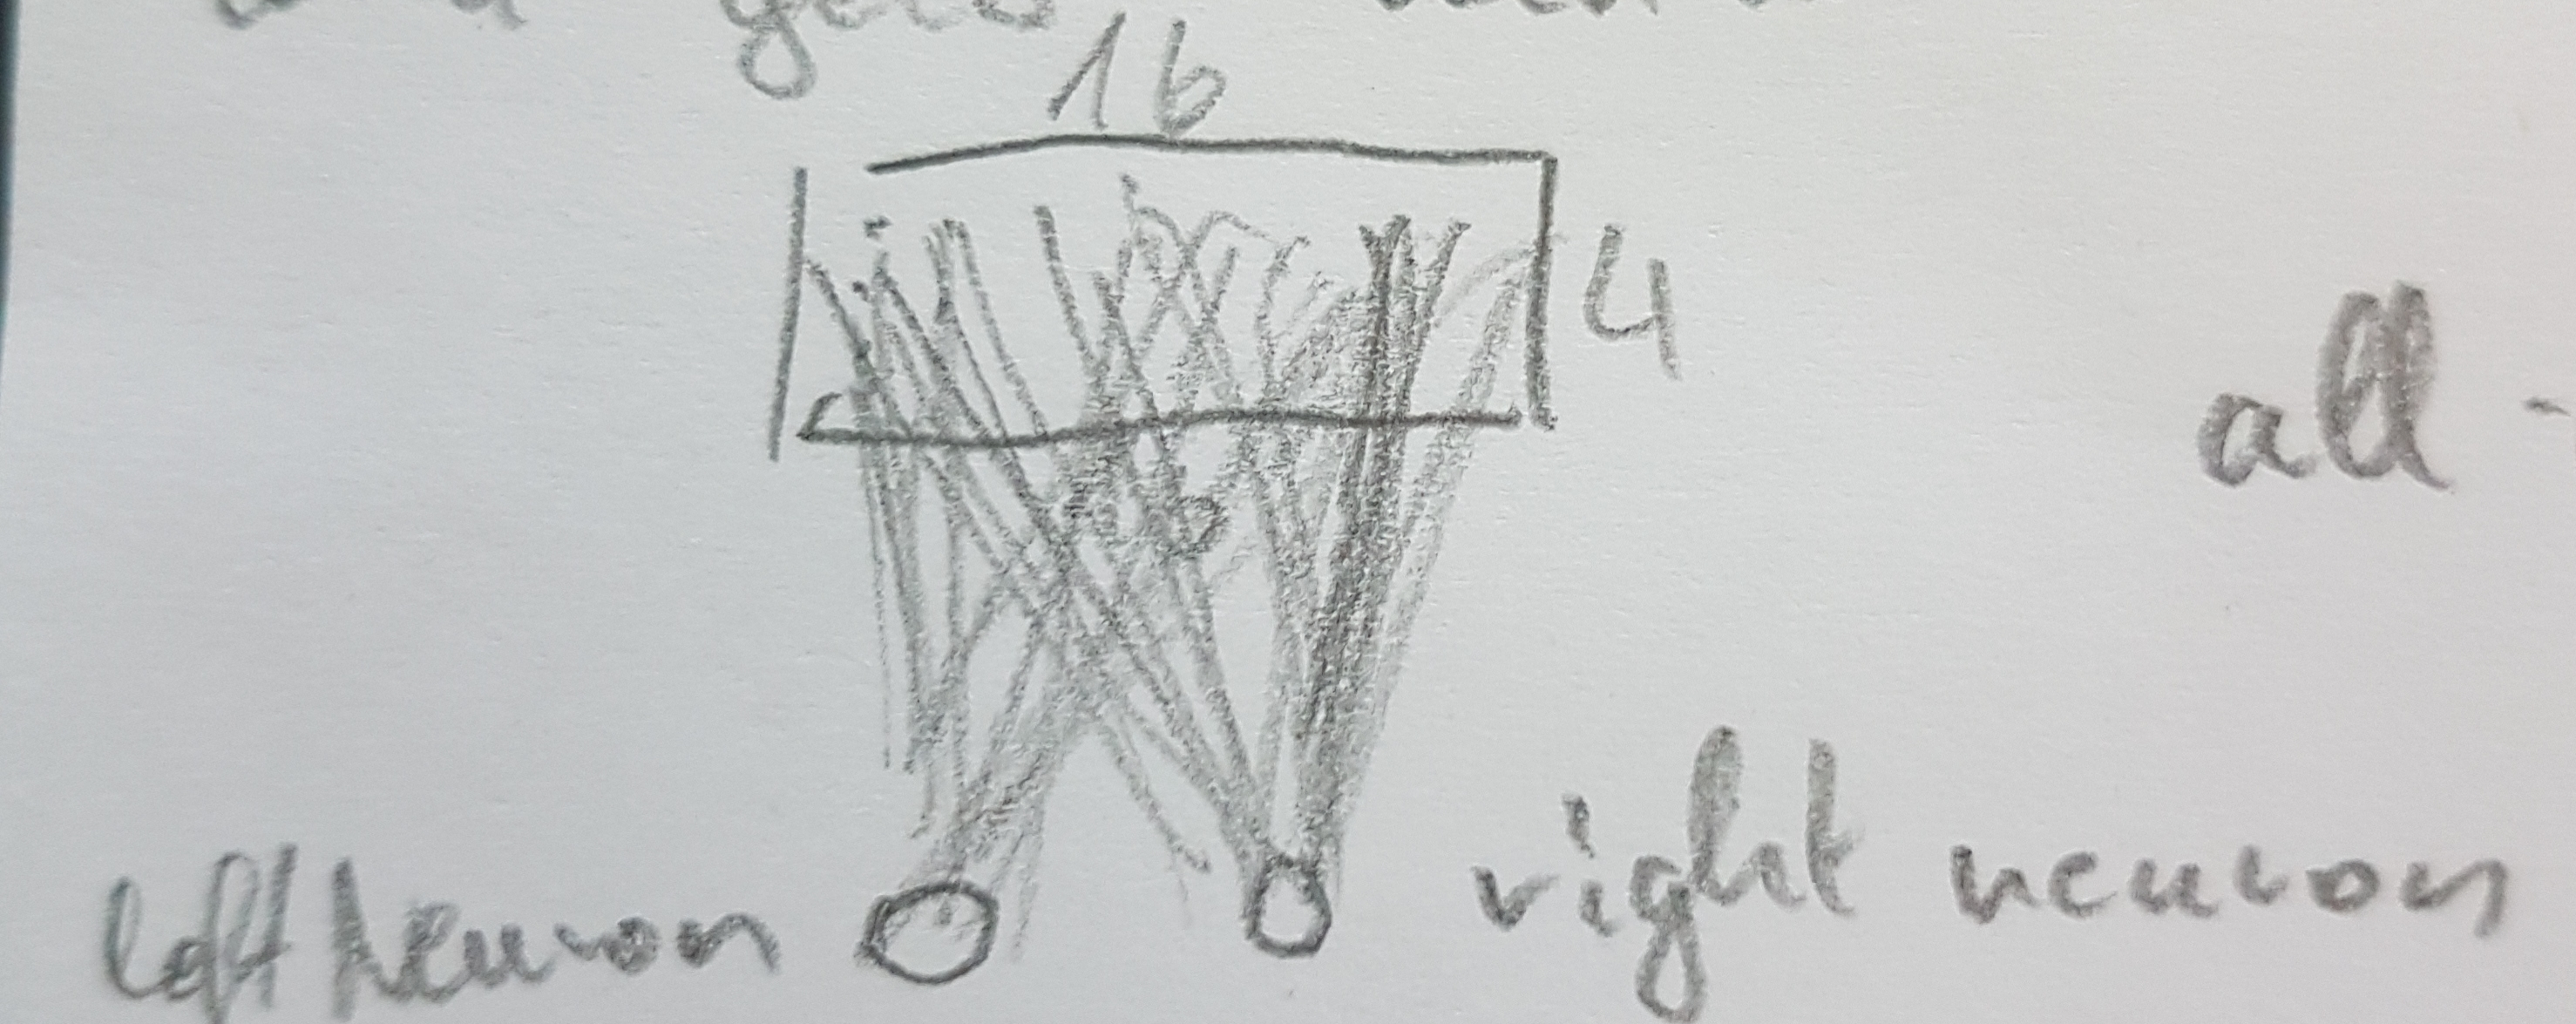
\includegraphics[width=\linewidth]{images/follow_arch.jpg}
	\caption{Target following snn architecture. 64 input neurons with all to all connections to 2 output neurons.}
	\label{fig:follw_arch}
\end{figure}

\begin{figure}
	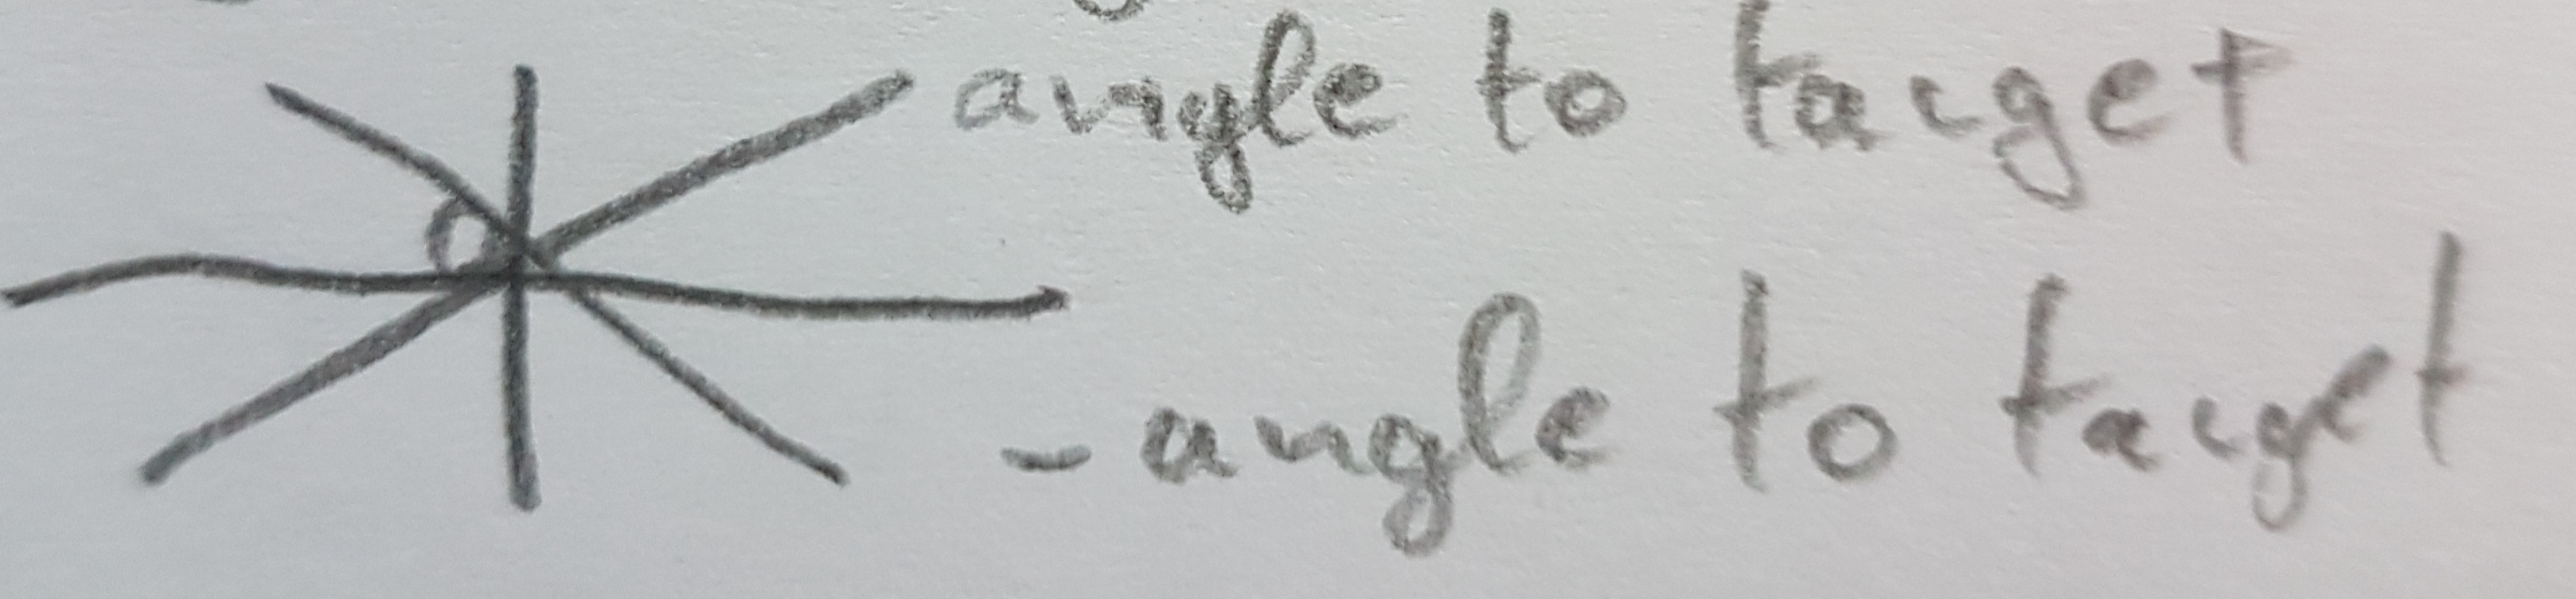
\includegraphics[width=\linewidth]{images/follow_rew.jpg}
	\caption{Reward function for the left and right neuron.}
	\label{fig:follw_rew}
\end{figure}

\section{Calculating the movement angle}

\begin{figure}
	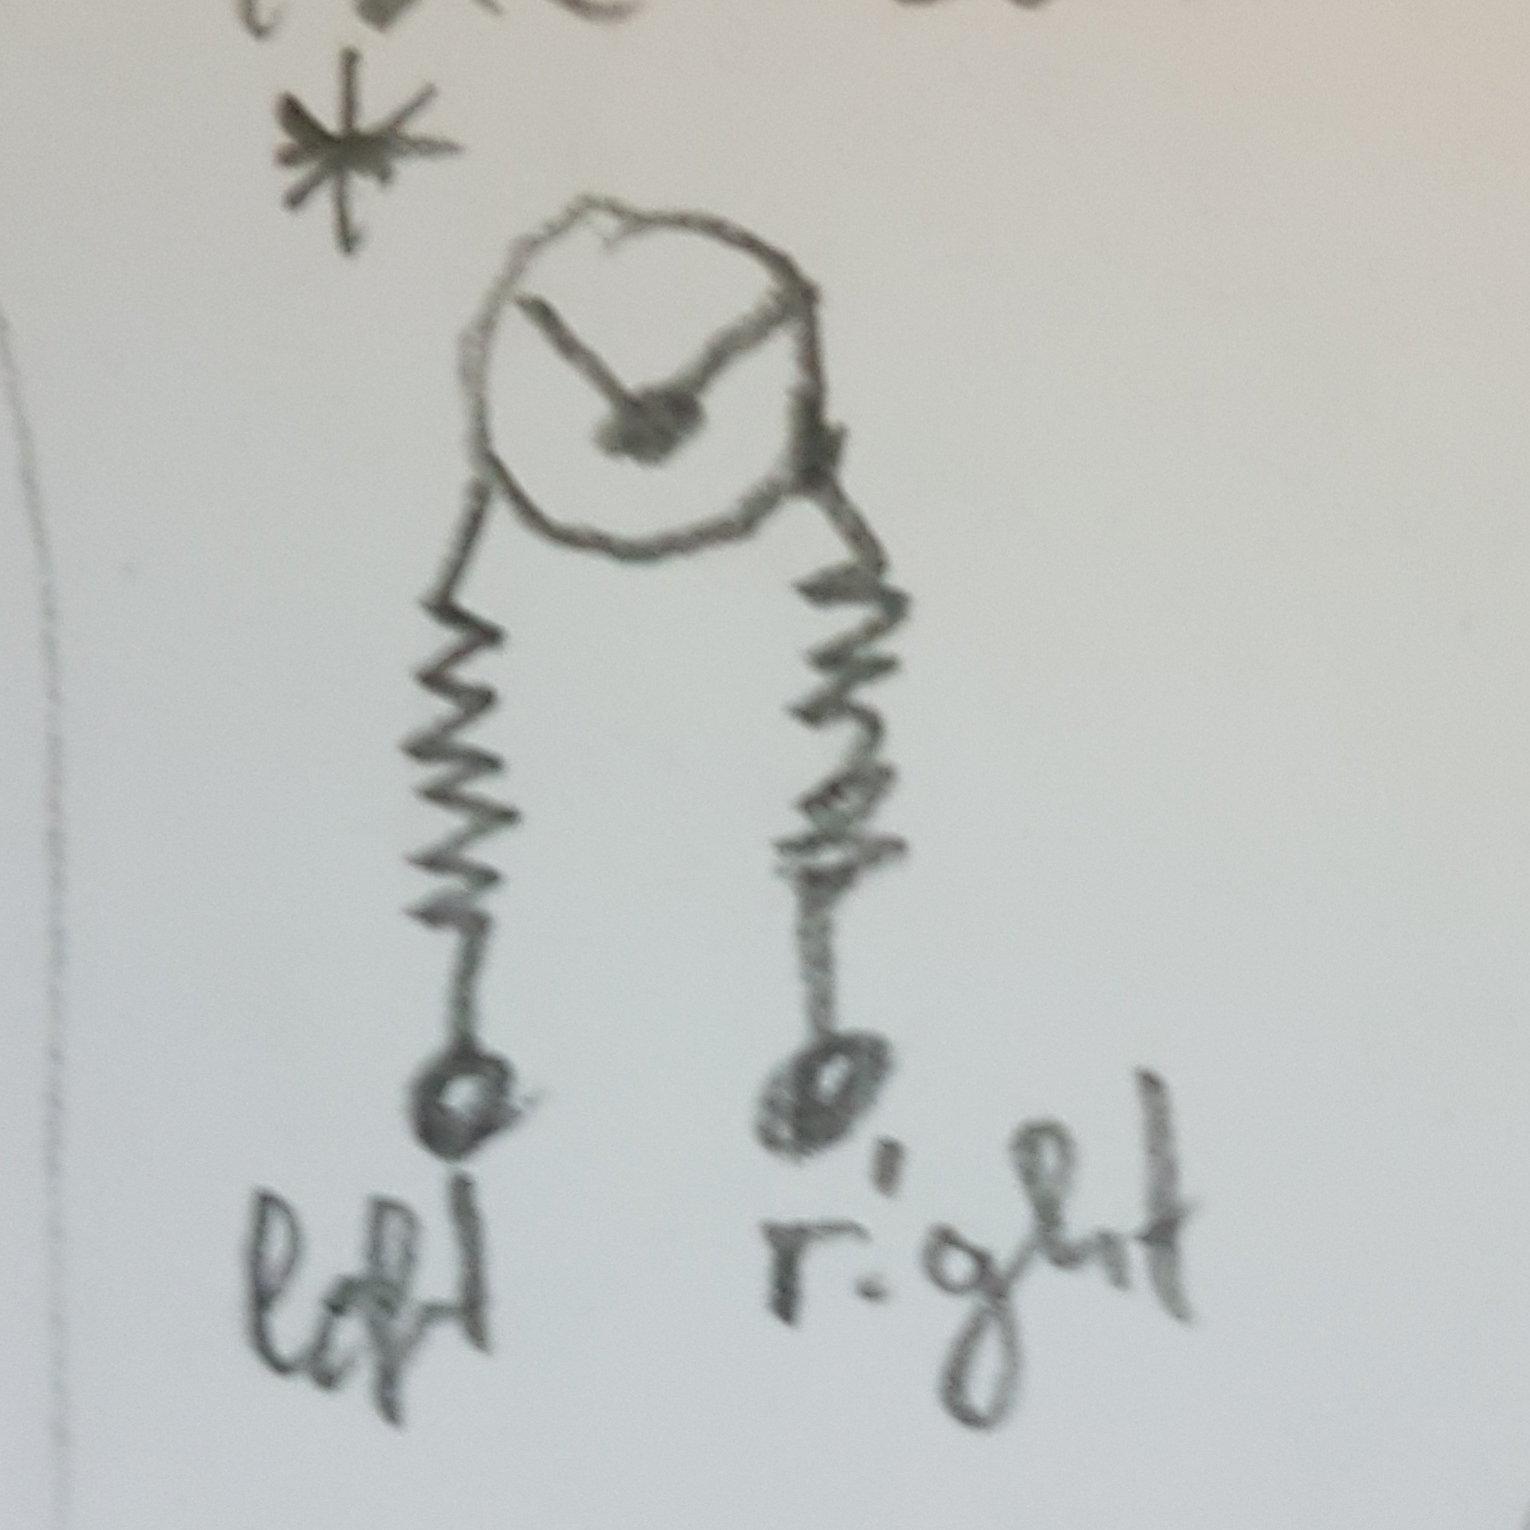
\includegraphics[width=\linewidth]{images/angle_model.jpg}
	\caption{Left and right neuron are muscles that compete.}
	\label{fig:angle_model}
\end{figure}

The output of the SNN gets normalised and interpreted as 2 competing muscles as shown in figure \ref{fig:angle_model}. Let $l_t$ and $r_t$ be the firing rate of the left and right neuron respectively at the time $t$ and let $ \alpha_{max} $ be the maximum right turn the snake can make. Then the angle $\alpha$ the snake should move is given by

% TODO check if it is l-r or r-l
\begin{equation}\label{eq:angle}
\alpha = \alpha_{max} \left(l_t - r_t\right)
\end{equation}

This angle is not given directly to the snake since that would lead to unstable movement. So we first take a combination parameteriset by $c \in \left[0; 1\right] $ of the angle from the last step and this step for the final angle.

\begin{equation}
\alpha_t = c \alpha + \left(1 - c\right) \alpha_{t-1}
\end{equation}

Where the $c$ gets calculated as follows
%TODO
\begin{equation}
c = \dots
\end{equation}

We use the angle from the last time step when $c$ is $0$ witch happens when there is no visual input. In that case it is good that the snake follows the last known angle to hopefully gain vision of the target again. We use the new angle if we have a lot of visual input. This model <insert name> was made by \ref{} for cars but most of the advantages are also there for the snake robot.

\section{Obstacle avoidance controller}

\begin{figure}
	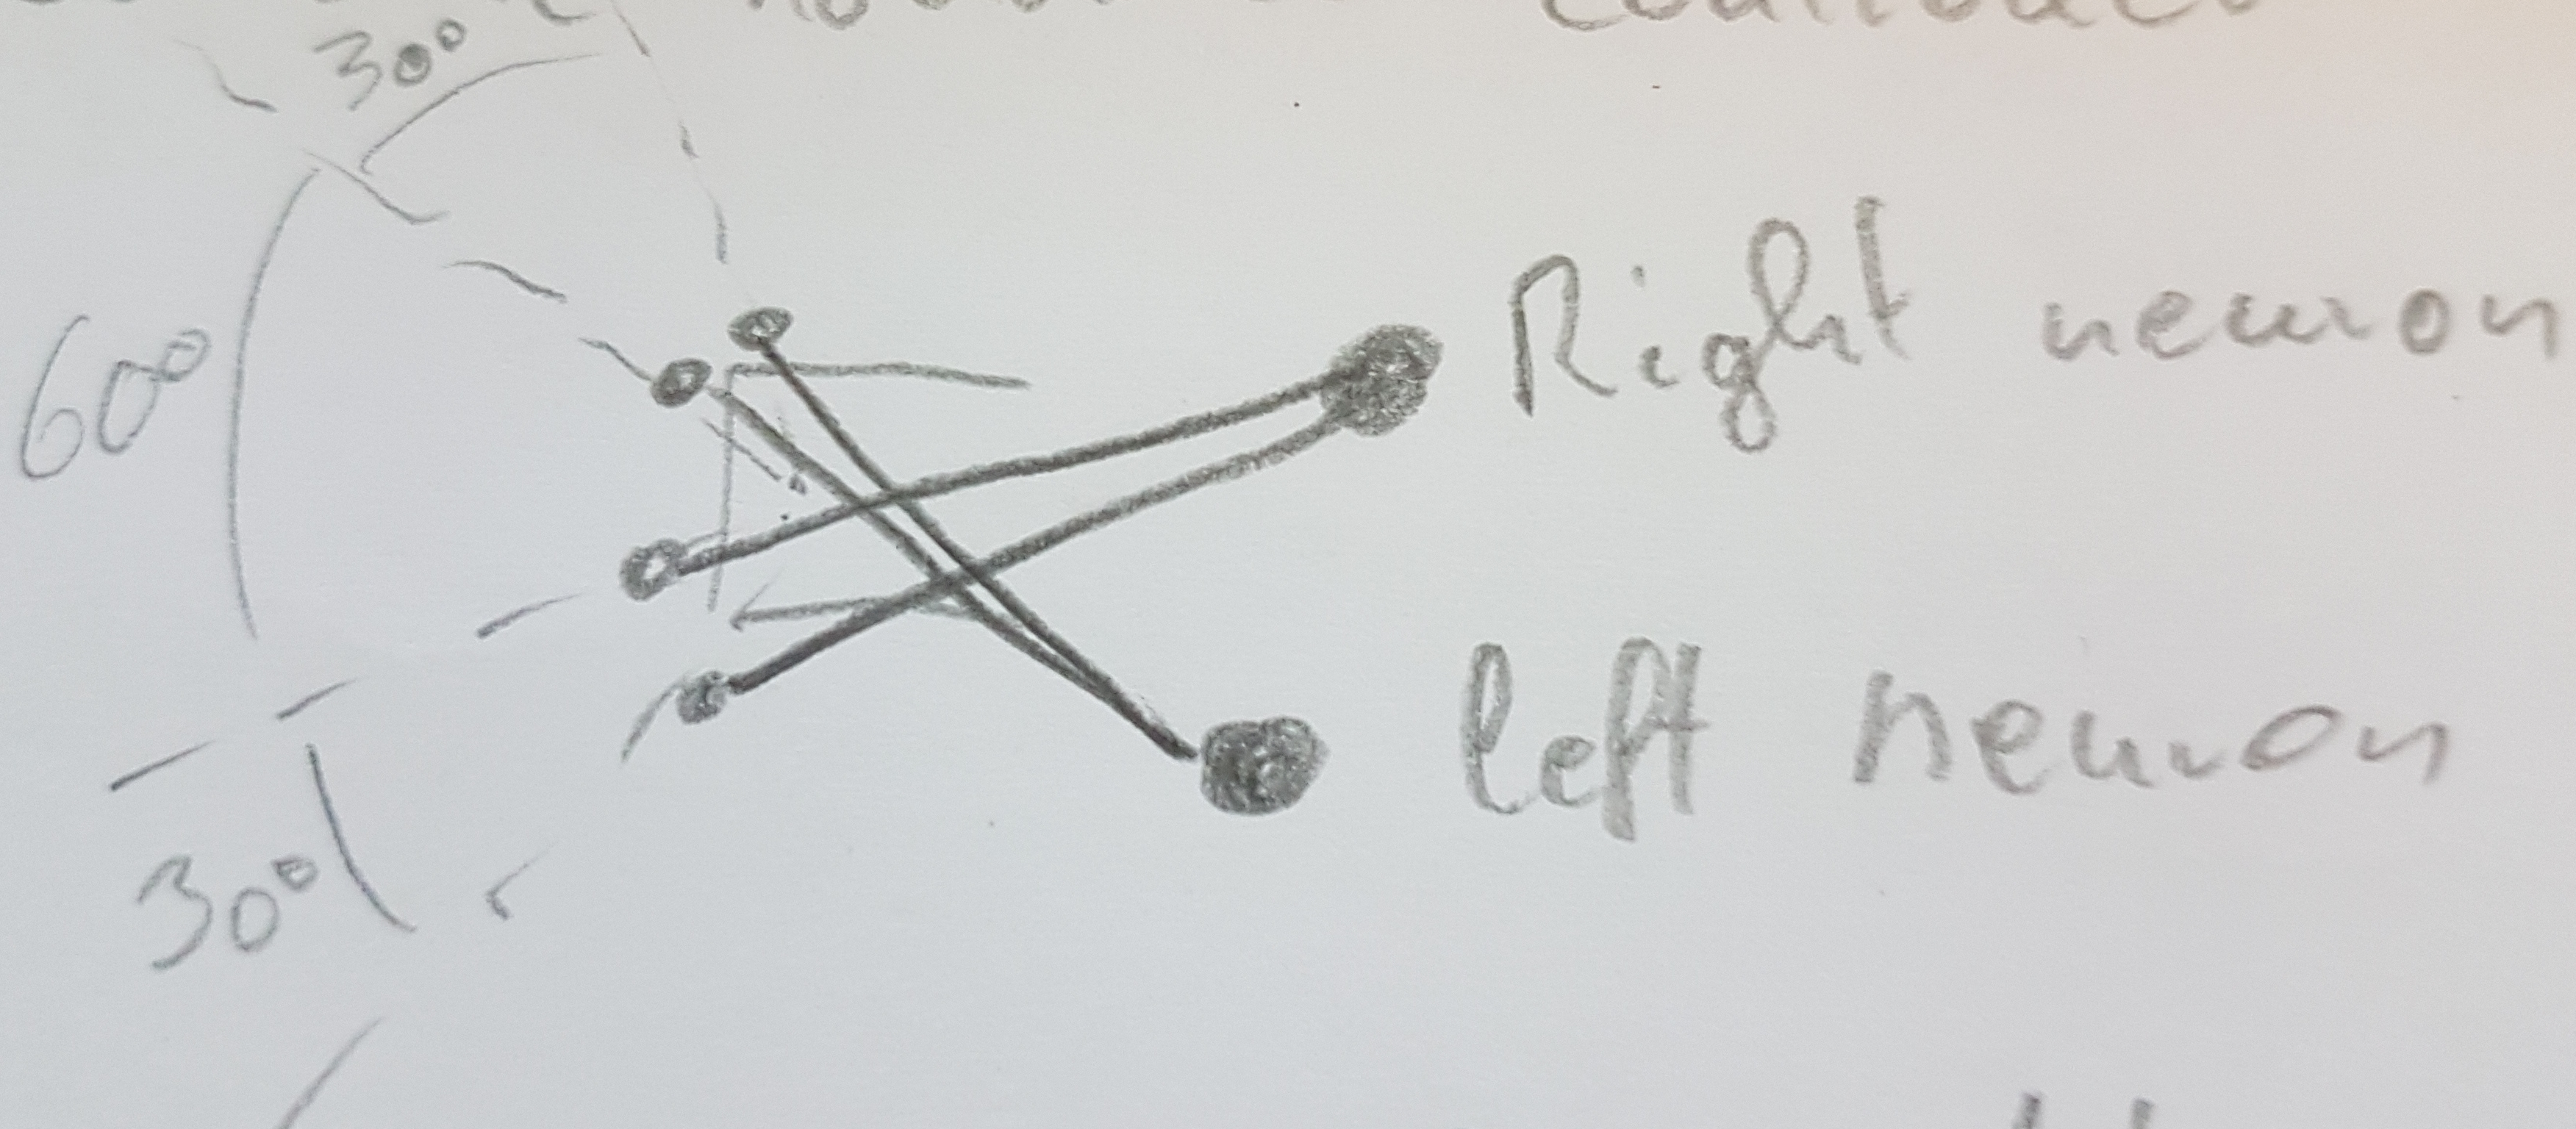
\includegraphics[width=\linewidth]{images/avoid_arch.jpg}
	\caption{Architecture of the obstacle avoidance controller.}
	\label{fig:avoid_arch}
\end{figure}
% formalize this shit
The obstacle avoidance controller makes sure the snake keeps a certain distance to obstacles. The network architecture is shown in figure \ref{fig:avoid_arch}. For this the 4 proximity sensors to the left and right of the snake are used. The preprocessing of the inputs goes as follows. First the maximum value gets assigned to a sensor if it senses nothing. Second there is a distance cut off after $3$m so everything farther away gets set to $3$. Next we divide by the maximum distance and take 1 minus that value as the input for the controller.
The left neuron gets connected to the right proximity sensors and the right neuron to the left proximity sensors. The reward gets assigned inividually and event based. In case of a collision both receive a positive reward of $1$. When no collision happens but the robot looses sight while avoiding an obstacle the side it was evading reveives a reward of $-1$ .

